\documentclass[11pt, a4paper]{article}
\usepackage{graphicx}
\usepackage{amsmath}
\usepackage{listings}
\usepackage{color}
\usepackage{fancyhdr}
\usepackage[utf8]{inputenc}
\usepackage[%  
    colorlinks=true,
    pdfborder={0 0 0},
    linkcolor=red
]{hyperref}

\definecolor{dkgreen}{rgb}{0,0.6,0}
\definecolor{gray}{rgb}{0.5,0.5,0.5}
\definecolor{mauve}{rgb}{0.58,0,0.82}

\lstset{frame=tb,
  language=Python,
  aboveskip=3mm,
  belowskip=3mm,
  showstringspaces=false,
  columns=flexible,
  basicstyle={\small\ttfamily},
  numbers=none,
  numberstyle=\tiny\color{gray},
  keywordstyle=\color{blue},
  commentstyle=\color{dkgreen},
  stringstyle=\color{mauve},
  breaklines=true,
  breakatwhitespace=true,
  tabsize=3
}



\title{EE2703-Assignment8}
\author{EE19B094}
\date{May 2021}

\setlength{\headheight}{15pt}
\pagestyle{fancy}
\fancyhf{}
\rhead{Assignment - 7}
\lhead{EE2703 - Applied Programming Lab}
\rfoot{Page \thepage}

\begin{document}

\maketitle
\newpage
\begin{abstract}
In this assignment, we analyse signals using the Fast Fourier transform. We do this by using the numpy.fft module.
\end{abstract}

\section{Accuracy of DFT}
To check how accurate the package is, we shall take the DFT of a sequence of random numbers, then take it’s IDFT and compare the two, as to how close they are.
\begin{lstlisting}
x=np.random.rand(100)
X=fft(x)
y=ifft(X)
c_[x,y]
maxError = max(np.abs(y-x))
print('Magnitude of maximum error between actual and computed values of the random sequence:', maxError)
\end{lstlisting}
The error is of the order of $10^{-15}$, which is usually good enough for our applications.

\section{DFT of various signals}
We calculate the DFT of various signals by first sampling the function at certain points and then using the fft() function on them. The function to do this is
\begin{lstlisting}
#Function to perform dft and plot spectrum
#Function to perform dft and plot spectrum
def perform_dft(func,N=512,steps = 513, r=4*np.pi, phase_limit=1e-3, xlim=40, w_lim=64):
	t = np.linspace(-r,r,steps)[:-1]	#Time range
	y = func_dict[func](t)				#Sampled function values
	Y = fftshift(fft(y))/N 				#Shifting freq
	w = np.linspace(-w_lim,w_lim,steps)[:-1]	#Frequency values to be plotted

	customplot(func,w,Y,xlim)
\end{lstlisting}
\subsection{Spectrum of sin(5t)}
We can write $$sin(5t) = \frac{1}{2j}(e^{5jt} - e^{-5jt})$$. Thus we expect peaks at $\omega = \pm 5$
\begin{lstlisting}
#Sin(5x) function
sin5 = lambda x : np.sin(5*x)

perform_dft('sin', xlim=10)
\end{lstlisting}

\begin{figure}[!tbh]
   	\centering
   	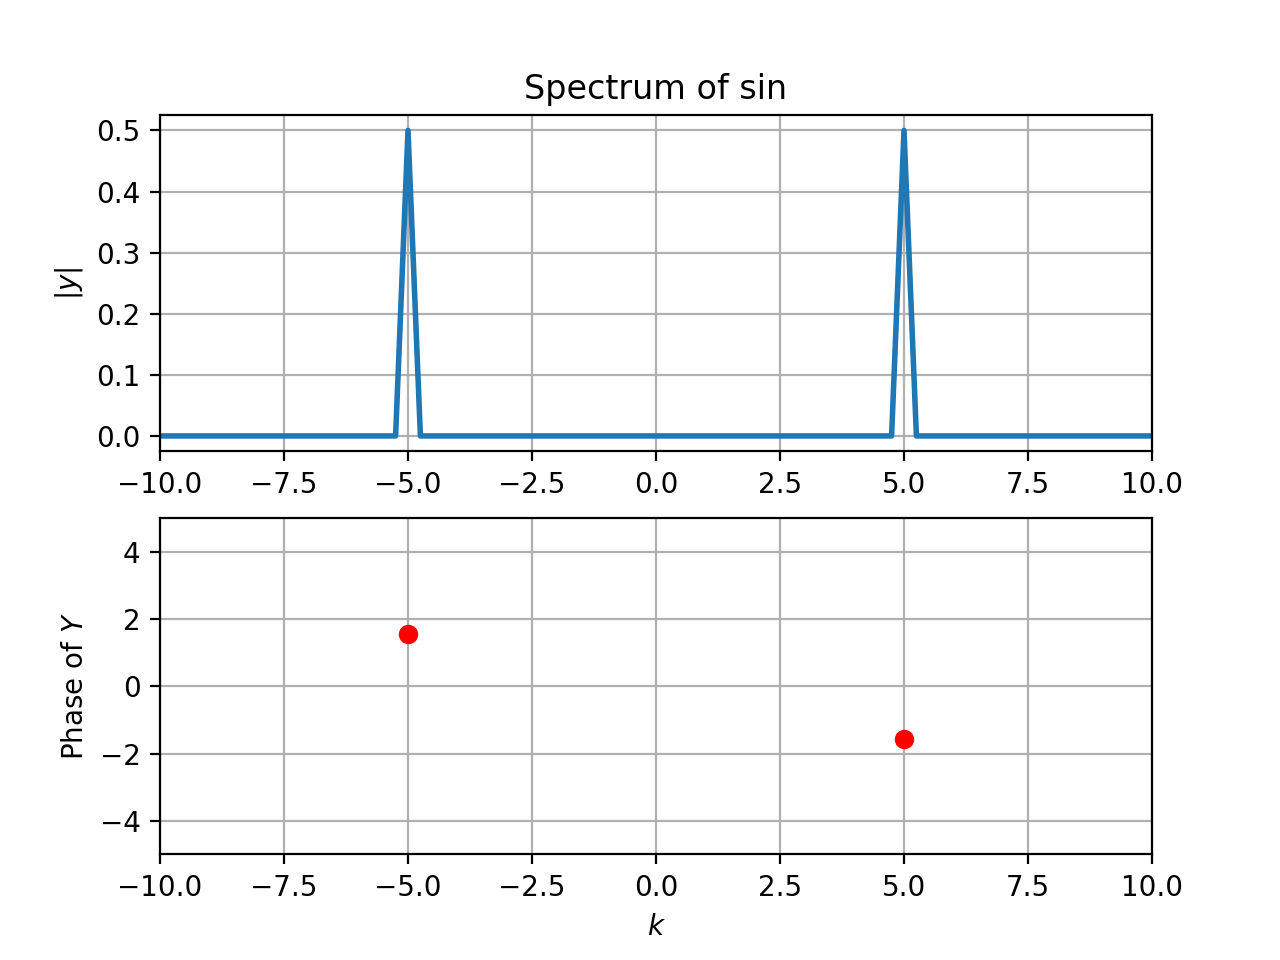
\includegraphics[scale=0.7]{sin.png}   
   	\caption{Sin(5t)}
   	\label{fig:Figure_1}
\end{figure}
\subsection{Amplitude modulated signal}
Our modulated signal is $(1 + 0.1cos(t))cos(10t)$ which can be rewritten as,
$$
(1 + 0.1cos(t))cos(10t)\ =\ \frac{1}{2}(e^{10jt} + e^{-10jt})\ +\ 0.1 \cdot \frac{1}{2} \cdot \frac{1}{2}(e^{11jt} + e^{-11jt} + e^{9jt} + e^{-9jt})
$$

We observe that the frequencies present in the signal are $\omega = \pm 10 , \omega = \pm 11 and \omega = \pm 9.$ Thus we expect the DFT also to have non-zero magnitudes only at these frequencies.
\begin{lstlisting}
#Modulated signal
modulated = lambda x : (1+0.1*np.cos(x))*np.cos(10*x)

perform_dft('modul',xlim=40)
\end{lstlisting}

\begin{figure}[!tbh]
   	\centering
   	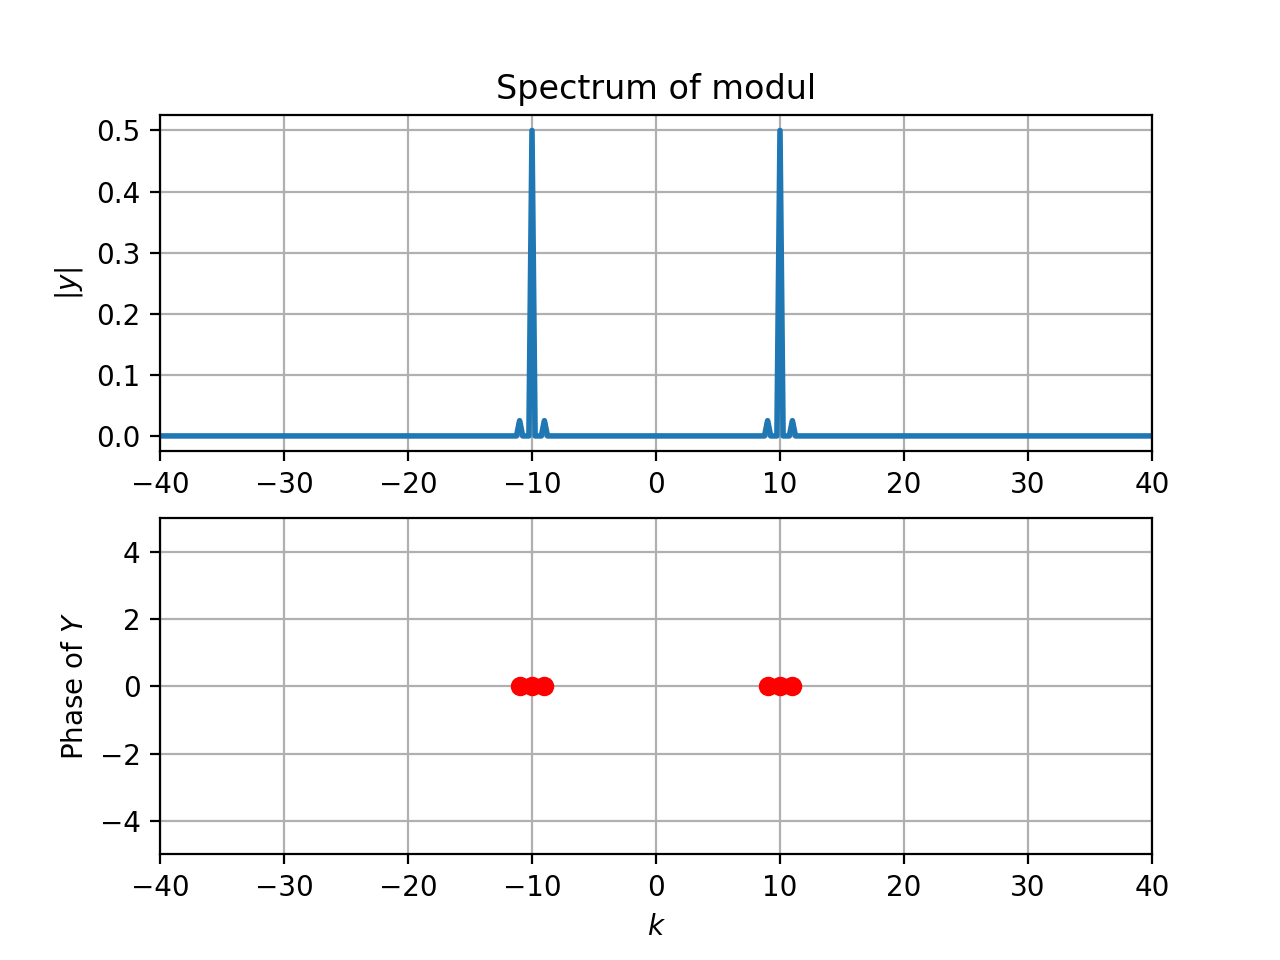
\includegraphics[scale=0.7]{AM.png}   
   	\caption{Amplituded modulated signal}
   	\label{fig:Figure_1}
\end{figure}
The magnitude has two large peaks at frequency of 10 corresponding to the carrier cosine wave. 

\subsection{Spectrum of $Sin^3(t)$ and $Cos^3(t)$}
Breaking down both the functions we get,
$$
sin^3(t) = \frac{3}{4}sin(t) - \frac{1}{4}sin(3t)
$$
Thus, here we would expect peaks at $\omega = \pm 1\ and\ \pm 3$ with bigger peaks at $\omega = \pm 1$
Similarly,
$$
cos^3(t) = \frac{3}{4}cos(t) + \frac{1}{4}cos(3t)
$$
Here too, we would expect peaks at $\omega = \pm 1\ and\ \pm 3$ with bigger peaks at $\omega = \pm 1$

\begin{lstlisting}
#Cos^3 function
cos3 = lambda x : np.cos(x)**3

#Sin^3 function
sin3 = lambda x : np.sin(x)**3

perform_dft('cos^3',xlim=15, steps= 129 , w_lim=16, N = 128)
perform_dft('sin^3',xlim=15)
\end{lstlisting}

\begin{figure}[!tbh]
   	\centering
   	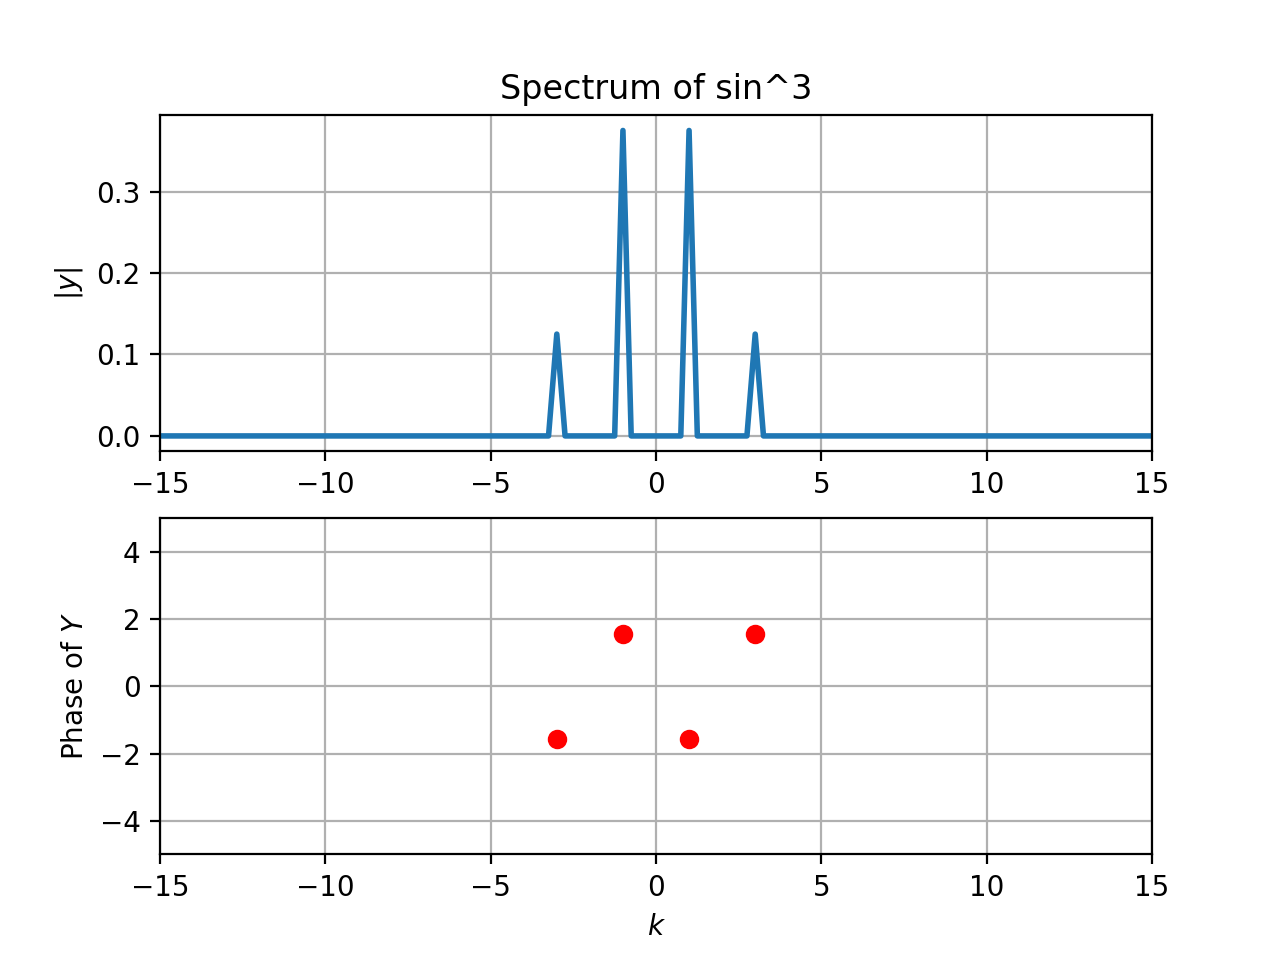
\includegraphics[scale=0.7]{sin3.png}   
   	\caption{$sin^3(x)$}
   	\label{fig:Figure_1}
\end{figure}
\begin{figure}[!tbh]
   	\centering
   	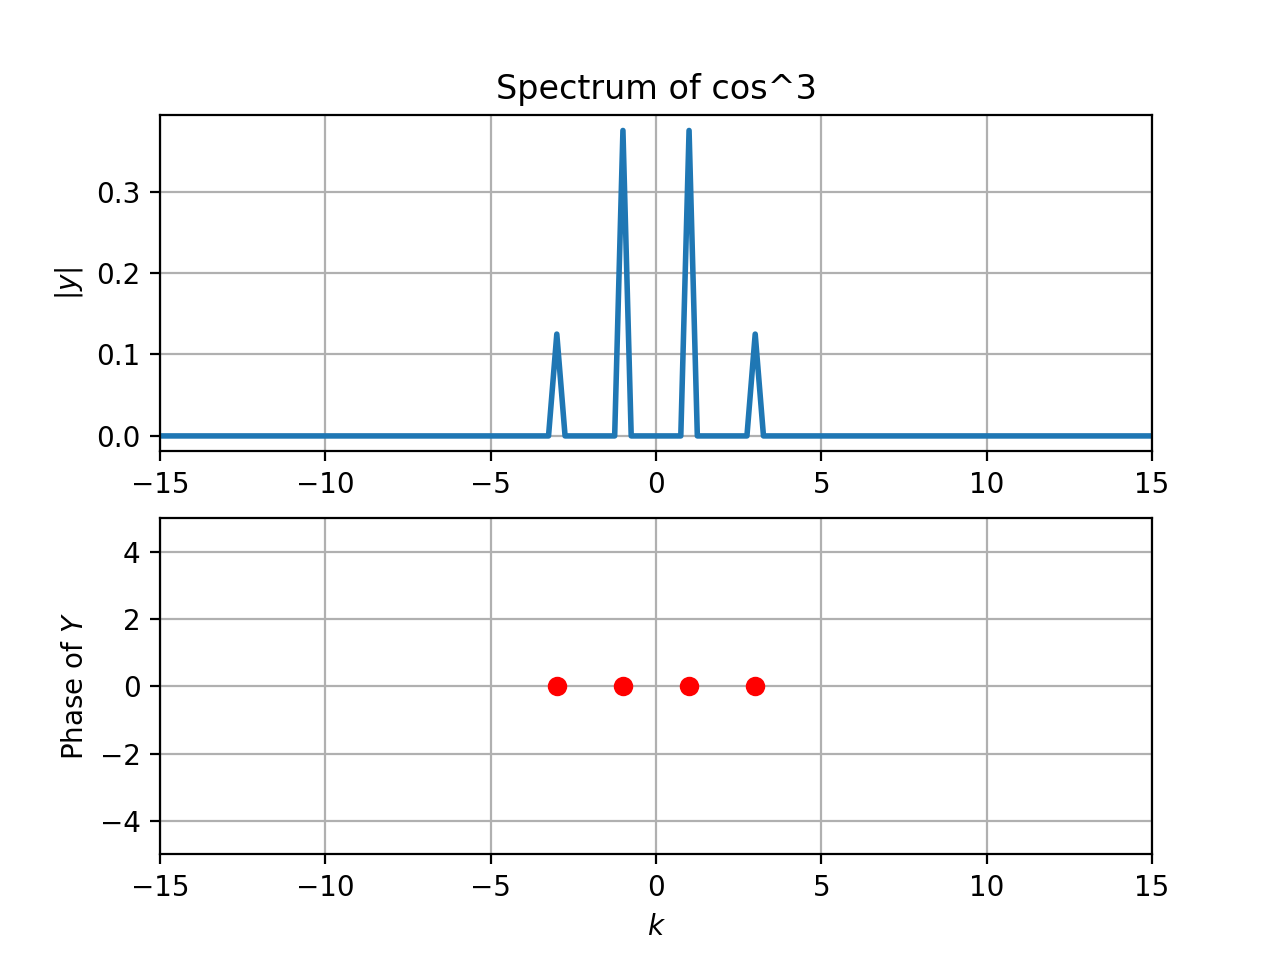
\includegraphics[scale=0.7]{cos3.png}   
   	\caption{$cos^3(x)$}
   	\label{fig:Figure_1}
\end{figure}

\subsection{Frequency modulated Signal}
The DFT of cos(20t + 5cos(t)) can be seen below:

\begin{lstlisting}
#cos(cos(x)) function 
coscos = lambda x : np.cos(20*x+5*np.cos(x))

perform_dft('coscos',xlim=40)
\end{lstlisting}

\begin{figure}[!tbh]
   	\centering
   	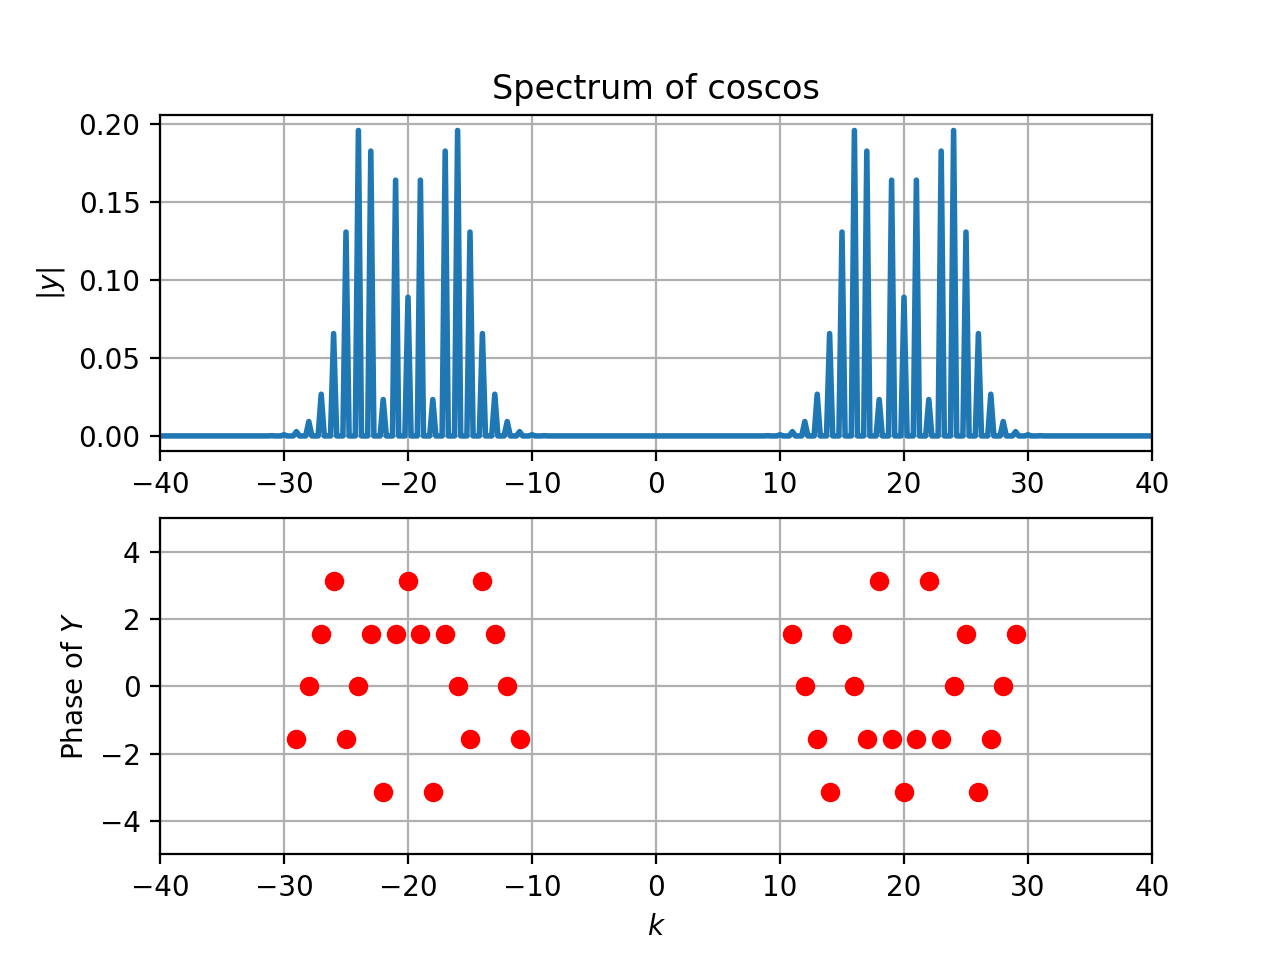
\includegraphics[scale=0.7]{FM.png}   
   	\caption{Frequency Modulated Signal}
   	\label{fig:Figure_1}
\end{figure}
There are many more sidebands compared to AM in the case of FM. Most of the energy of the signal is also present in these sidebands rather than the carrier band in the case of AM.

\subsection{Gaussian Signal}
A function to estimate the DFT of the gaussian is shown below. The function iteratively increases window size and sample number until the consecutive total absolute error between estimates reduces below a given threshold.
\begin{lstlisting}
def perform_dft_gaussian(func,tolerance=1e-6,N=128):
	T = 8*np.pi
	Y_old = 0

	while 1:

		#Time resolution
		dt = T/N
		#Frequency resolution
		dw = 2*np.pi/T

		#Freq window size
		W = N*dw

		#Time samples
		t = np.linspace(-T/2,T/2,N+1)[:-1]
		#Freq samples
		w = np.linspace(-W/2,W/2,N+1)[:-1]

		y = gauss(t)
		Y_new = dt/(2*np.pi) * fftshift(fft(ifftshift(y)))
		error = sum(abs(Y_new[::2]) - Y_old)
		Y_old = Y_new

		if error < tolerance:
			customplot(func,w,Y_new,5)
			print("Error in Gaussian case is {}".format(error))
			return

		T*=2
		N*=2

perform_dft_gaussian('gauss')
\end{lstlisting}

\begin{verbatim}
    Error in Gaussian case is (2.59763998505802e-15+0j)
\end{verbatim}
\begin{figure}[!tbh]
   	\centering
   	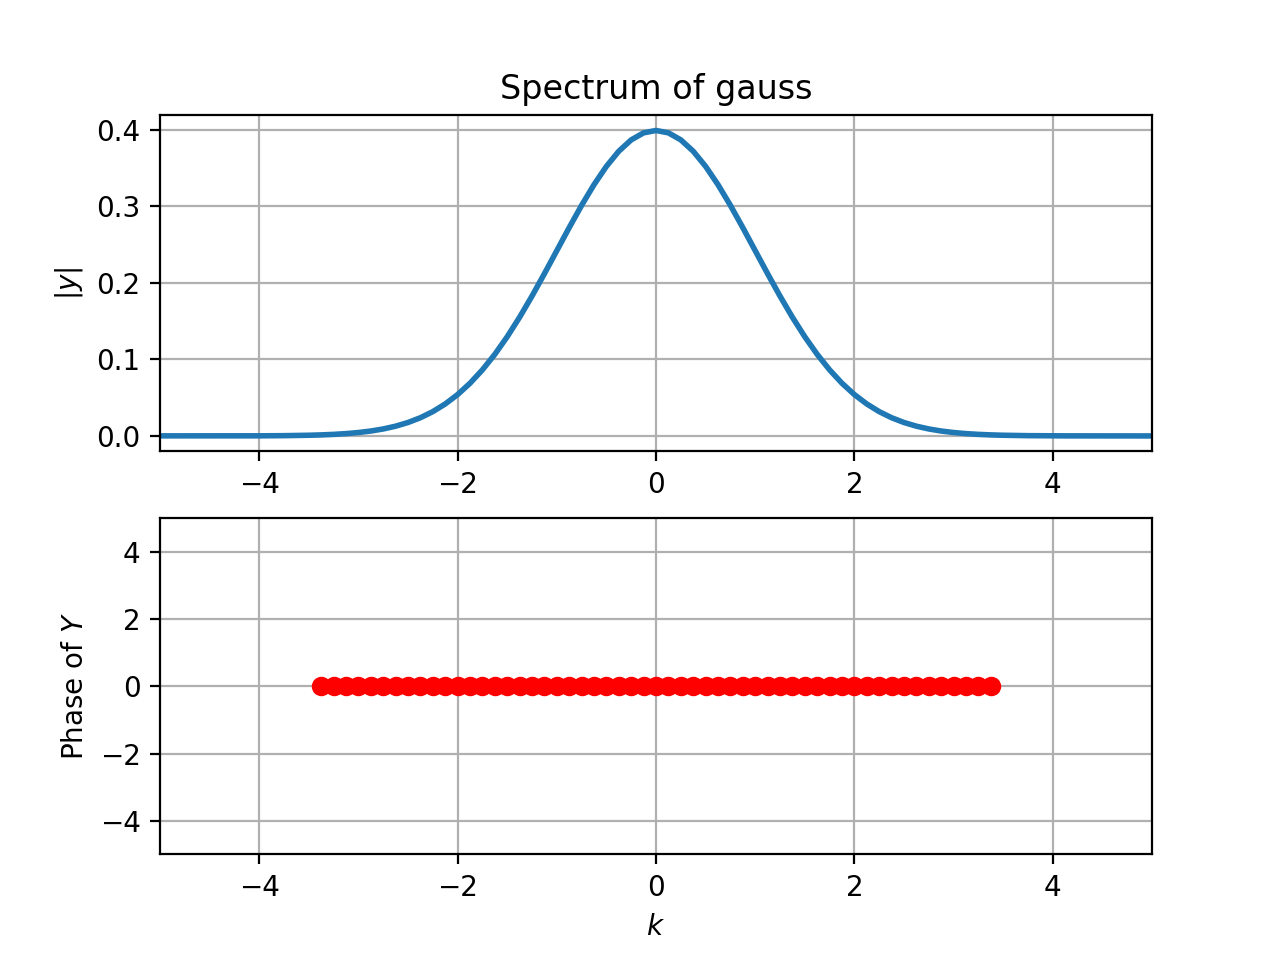
\includegraphics[scale=0.7]{gaussian.png}   
   	\caption{Frequency Modulated Signal}
   	\label{fig:Figure_1}
\end{figure}

\newpage
\section{Observations}
For the spectrums of the functions other than gaussian curve, we could break the signal into sinusodials and thus we could predict the DFT.\newline

However, from the gaussain we saw that with a sufficiently large window size and sampling rate, the DFT approximates the CTFT of the gaussian.
This is because the magnitude of the gaussian quickly approaches 0 for large values of time. This means that there is lesser frequency domain aliasing due to windowing.

\section{Conclusion}
Thus, in this assignment we used the numpy.fft package to simulate the DFT of some standard functions and carried out their frequency component analysis.

\end{document}
